\chapter{Natuurlijke Deductie en Sequenten}
Een alternatief om logische gevolgtrekking te bewijzen is met behulp van \emph{sequenten-calculus}, en het daaraan gerelateerde systeem van \emph{natuurlijke deductie}. Beide formalismen in dit hoofdstuk volgen uit het werk van Gentzen, die poogde een bewijssysteem te formaliseren dat niet, zoals Hilbert's eerdere systeem, van onvoorwaardelijke tautologi\"en afhankelijk was. Van de twee is sequent-calculus vaak eenvoudiger om een stelling mee te bewijzen, met name omdat de bewijzen meer lineair opgebouwd worden. Natuurlijke deductie vergt wat meer creativiteit, omdat je meer van twee kanten naar elkaar toe moet werken, en heeft de mogelijkheid net iets compactere bewijzen te leveren. Natuurlijke deductiebewijzen hebben daarnaast een interessante link naar programma's en types, in het bijzonder in de functionele stijl. Deze link komt in Sectie~\ref{sec:curry-howard} verder aan bod.

In beide systemen wordt gewerkt met \emph{sequenten}, oftewel voorwaardelijke tautologi\"en. De sequent $\Gamma \vdash \Delta$ of $\Gamma \implies \Delta$\sidenote{De eerste notatie is gebruikelijker voor natuurlijke deductie, de tweede voor sequenten-calculus.} geeft bijvoorbeeld aan dat, zolang de antecedent $\Gamma$ een tautologie is, de consequent $\Delta$ dat ook moet zijn. Een bewijs begint bovenaan met een aantal axioma's, doorgaans van de vorm $A \implies A$; hier worden regels op toegepast om uiteindelijk op de te bewijzen stelling uit te komen. Om een dergelijk bewijs te schrijven begin je doorgaans onderaan en probeer je door het toepassen van de juiste regels op enkel axioma's uit te komen. In dit geval is de stelling onvoorwaardelijk bewezen. Als het niet mogelijk is een bewijs op deze manier te completeren, dan is de stelling op z'n minst afhankelijk bewezen door de overgebleven antecedenten als aannames toe te voegen. 

  \begin{marginfigure}
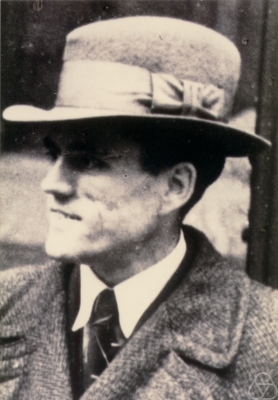
\includegraphics[width=0.6\textwidth]{gentzen.jpg}\\
    Gerhard Gentzen {\scriptsize\emph (Image by Wikipedia)}\\[3mm]
  \end{marginfigure}

\section{Sequenten-calculus}
In het geval van de sequenten-calculus mogen sequenten nul of meerdere antecedenten en consequenten hebben, bijvoorbeeld $A_0, A_1, \dots, A_n \implies B_0, B_1, \dots, B_n$. We interpreteren deze sequent zo dat als elke $A_i$ waar is, tenminste een $B_i$ waar moet zijn.

De regels die we mogen toepassen staan gegeven in Stelling~\ref{th:lk}. De regels zijn onder te verdelen in \emph{structurele regels} (weakening, contraction en exchange), die enkel de structuur van het bewijs veranderen, en \emph{logische regels} die logische connectieven introduceren. De laatste categorie is verder te verdelen in \emph{linker-} en \emph{rechter-regels}, afhankelijk van welke kant van de pijl ze opereren.

\begin{figure}[ht]
\begin{theorem}\label{th:lk} Gentzen Calculus \lk
\paragraph{Axioma's}\mbox{}\\[3mm]
\inference{Ax}{}{A \implies A} (voor atomaire $A$)
\hspace{5mm}
\inference{L\bot}{}{\bot \implies}
\hspace{5mm}
\inference{R\top}{}{\implies \top}

\paragraph{Structurele regels}\mbox{}\\[3mm]
\inference{LW}{\Gamma, \Gamma^\prime \implies \Delta}{\Gamma, A, \Gamma^\prime \implies \Delta}
\hspace{5mm}
\inference{RW}{\Gamma \implies \Delta, \Delta^\prime}{\Gamma \implies \Delta, A, \Delta^\prime}

\vspace{5mm}

\inference{LC}{\Gamma, A, A, \Gamma^\prime \implies \Delta}{\Gamma, A, \Gamma^\prime \implies \Delta}
\hspace{5mm}
\inference{RC}{\Gamma \implies \Delta, A, A, \Delta^\prime}{\Gamma \implies \Delta, A, \Delta^\prime}

\vspace{5mm}

\inference{LE}{\Gamma, A, B, \Gamma^\prime \implies \Delta}{\Gamma, B, A, \Gamma^\prime \implies \Delta}
\hspace{5mm}
\inference{RE}{\Gamma \implies \Delta, A, B, \Delta^\prime}{\Gamma \implies \Delta, B, A, \Delta^\prime}

\vspace{5mm}

\fork{Cut}{\Gamma \implies A, \Delta}{\Sigma, A \implies \Pi}{\Gamma, \Sigma \implies \Delta, \Pi}

\paragraph{Logische regels}\mbox{}\\[3mm]

\fork{L\to}{\Gamma \implies A, \Delta}{B, \Gamma^\prime \implies \Delta^\prime}{\Gamma, A \to B, \Gamma^\prime \implies \Delta, \Delta^\prime}
\hspace{5mm}
\inference{R\to}{\Gamma, A \implies B, \Delta}{\Gamma \implies A \to B, \Delta}

\vspace{5mm}

%\inference{L\land_1}{\Gamma, A \implies \Delta}{\Gamma, A \land B \implies \Delta}
%\hspace{5mm}
%\inference{L\land_2}{\Gamma, B \implies \Delta}{\Gamma, A \land B \implies \Delta}
\inference{L\land}{\Gamma, A, B, \Gamma^\prime \implies \Delta}{\Gamma, A \land B, \Gamma^\prime \implies \Delta}
\hspace{5mm}
\fork{R\land}{\Gamma \implies \Delta, A, \Delta^\prime}{\Gamma \implies \Delta, B, \Delta^\prime}{\Gamma \implies \Delta, A \land B, \Delta^\prime}

\vspace{5mm}

\fork{L\lor}{\Gamma, A, \Gamma^\prime \implies \Delta}{\Gamma, B, \Gamma^\prime \implies \Delta}{\Gamma, A \lor B, \Gamma^\prime \implies \Delta}
\hspace{5mm}
%\inference{R\lor_1}{\Gamma \implies \Lambda, A, \Delta}{\Gamma \implies \Lambda, A \lor B, \Delta}
%\hspace{5mm}
%\inference{R\lor_2}{\Gamma \implies \Lambda, B, \Delta}{\Gamma \implies \Lambda, A \lor B, \Delta}
\inference{R\lor}{\Gamma \implies \Delta, A, B, \Delta^\prime}{\Gamma \implies \Delta, A \lor B, \Delta^\prime}

\vspace{5mm}

\inference{L\neg}{\Gamma \implies A, \Delta}{\Gamma, \neg A \implies \Delta}
\hspace{5mm}
\inference{R\neg}{\Gamma, A \implies \Delta}{\Gamma \implies \neg A, \Delta}
\end{theorem}
\end{figure}

%\paragraph{Rules for Quantifiers}\mbox{}\\[3mm]
%\inference{L\forall}{\Gamma, A[t/x], \Sigma \implies \Delta}{\Gamma, \forall x A, \Sigma \implies \Delta}
%\hspace{5mm}
%\inference{R\forall}{\Gamma \implies \Lambda, A[z/x], \Theta}{\Gamma \implies \Lambda, \forall x A, \Theta}
%
%\vspace{5mm}
%
%\inference{L\exists}{\Gamma, A[z/x], \Sigma \implies \Delta}{\Gamma, \exists x A, \Sigma \implies \Delta}
%\hspace{5mm}
%\inference{R\exists}{\Gamma \implies \Lambda, A[t/x], \Theta}{\Gamma \implies \Lambda, \exists x A, \Theta}


\subsection{Voorbeelden}
We beginnen met een eenvoudig voorbeeld, en zullen daarna een iets groter gevolg bewijzen.

\begin{example}\label{ex:lk:helloworld}
Geef een afleiding in \lk{} voor de sequent $P \land Q \implies P$.

We beginnen met hetgeen we willen bewijzen als eindsequent:

\begin{prooftree}
\lksorry{$P \land Q \implies P$}
\end{prooftree}

Nu moeten we op zoek naar een afleidingsregel met de juiste sequent onder de streep. Dit kan eigenlijk altijd een structurele regel zijn, maar deze werken eigenlijk alleen om een sequent in een andere vorm te schrijven, dus we proberen eerst de logische regels. Als we een logische regel vinden die \emph{net niet} past, dan kunnen we op zoek naar een structurele regel als \enquote{adapter}. In dit geval is er maar \'e\'en logisch connectief, een $\land$ links, dus zouden we de $L\land$ regel kunnen proberen:

\begin{prooftree}
  \lksorry[$L\land$]{$P \land Q \implies P$}
\end{prooftree}

Nu kunnen we boven de streep invullen. De Griekse letters staan voor een set logische zinnen; in het geval van $\Gamma$ is deze leeg omdat er niets anders links van de pijl staat. $A$ en $B$ in de regel komen overeen met $P$ en $Q$ in onze formule. $\Delta$ staat in deze regel voor alles achter de pijl, in ons geval $P$. Aan $\Gamma$ en $\Delta$ verandert er niets, maar links van de komma splitsen we $P \land Q$ op in de losse zinnen $P$ en $Q$. Als we dit in het template invullen krijgen we de volgende situatie:

\begin{prooftree}
\lksorry{$P, Q \implies P$}
\lklconj{$P \land Q \implies P$}
\end{prooftree}

Nu is het tijd om een structurele regel toe te passen. We zij bijna willen toe naar het axioma $P \implies P$, maar we moeten nog van de $Q$ af zien te komen. Dit kan met weakening links, waarbij de $A$ onder de streep de in ons geval $Q$ is. Na toepassen van de regel zijn we deze boven de streep vergeten:

\begin{prooftree}
\lksorry{$P \implies P$}
\lklcontr{$P, Q \implies P$}
\lklconj{$P \land Q \implies P$}
\end{prooftree}

Nu we een Axioma hebben hoeven we deze alleen nog te markeren en is ons bewijs klaar:

\begin{prooftree}
\lkax{$P \implies P$}
\lklcontr{$P, Q \implies P$}
\lklconj{$P \land Q \implies P$}
\end{prooftree}
\hfill\qed

\end{example}

\begin{example}\label{ex:lk:trans}
Laten we nu kijken naar een iets groter voorbeeld: $P \to Q, Q \to R \implies P \to R$, oftewel als $P$ voldoende is om $Q$ aan te tonen, en $Q$ voldoende is om $R$ aan te tonen, dan kunnen we $P$ als direct bewijs voor $R$ gebruiken. Voor dit bewijs zullen we ons voor de tussenstappen tot de logische regels beperken. De structurele regels worden wel meegenomen, maar niet als losse stappen in de uitleg.

\begin{prooftree}
\lksorry{$P \to Q, Q \to R \implies P \to R$}
\end{prooftree}

  We beginnen wederom met de te bewijzen sequent onder de streep. In dit bewijs hebben we drie connectieven om mee aan de slag te gaan, specifiek drie implicaties. Als we kijken naar de regels uit Stelling~\ref{th:lk}, dan zien we dat $R\!\to$ eenvoudiger oogt dan $L\!\to$, dus dat zou een logisch begin zijn. In plaats van te splitsen hoeven we enkel het antecedent van de implicatie naar links te halen:

\begin{prooftree}
\lksorry{$P \to Q, Q \to R, P \implies R$}
\lkrimpl{$P \to Q, Q \to R \implies P \to R$}
\end{prooftree}

Nu hebben we nog twee operatoren over, de implicaties aan de rechterkant. Voor de $L\!\to$ regel moeten we een beetje schuiven om de juiste termen aan de juiste kant te krijgen, maar met een enkele exchange kunnen we $Q \to R$ splitsen. We krijgen dan links $Q$ als consequent en rechts $R$ als antecedent. Dit geeft de sequenten $P \to Q, P \implies Q$ en $R \implies R$. Dat zou moeten lukken.

\begin{prooftree}
  \lksorry{$P \to Q, P \implies Q$}

  \lkax{$R \implies R$}

\lklimpl{$P \to Q, P, Q \to R \implies R$}
\lklexch{$P \to Q, Q \to R, P \implies R$}
\lkrimpl{$P \to Q, Q \to R \implies P \to R$}
\end{prooftree}

Rechts zijn we meteen klaar, dus rest ons de linkerkant. Deze sequent is een enkele exchange verwijderd van een modus ponens, $P, P \to Q \implies Q$. Om deze weg te werken gebruiken we nogmaals de $L\to$ regel, die ons bij de laatste twee axioma's brengt:

\begin{prooftree}
    \lkax{$P \implies P$}

    \lkax{$Q \implies Q$}

  \lklimpl{$P, P \to Q \implies Q$}
  \lklexch{$P \to Q, P \implies Q$}

  \lkax{$R \implies R$}

\lklimpl{$P \to Q, P, Q \to R \implies R$}
\lklexch{$P \to Q, Q \to R, P \implies R$}
\lkrimpl{$P \to Q, Q \to R \implies P \to R$}
\end{prooftree}
\hfill\qed
\end{example}

%We zien hier dat de structurele stappen in een sequentenbewijs een fors deel van de totale  afleiding kunnen zijn. Om bewijzen iets te versimpelen bestaan er alternatieve formulaties van de sequenten-calculus, waar logische zinnen niet in een lijst, maar in een multiset worden beschouwd. In degrelijke formulaties is de volgorde niet langer van belang. Voor klassieke logica kunnen we zelfs nog verder gaan en ook weakening en contraction stilzwijgend negeren, maar verderop zullen we zien dat deze regels wel degelijk betekenis hebben als we in Hoofdstuk~\ref{ch:systemen} logische systemen gaan tegenkomen die deze stappen niet zonder meer toelaten.

\subsection{De cut-regel}
De cut-regel is een zekere zin discutabel. Elke stelling die met cut bewezen kan worden, kan ook zonder cut worden bewezen. De set van geldige stellingen verandert dus niet door deze regel toe te voegen, en in principe heeft een systeem met zo min mogelijk regels de voorkeur. Desalniettemin kan de cut-regel helpen om proofs overzichtelijk te houden. Beschouw de twee bewijzen van het sequent $A \land B, \neg A \lor C \implies C$ hieronder.

\begin{prooftree}
  \lkax{$A\implies A$}
  \lklweak{$A, B \implies A$}
  \lklconj{$A \land B \implies A$}

    \lkax{$A\implies A$}
    \lklneg{$A, \neg A\implies$}
    \lklweak{$A, \neg A \implies C$}

    \lkax{$C \implies C$}
    \lklweak{$A, C \implies C$}
  \lkldisj{$\neg A \lor C, A \implies C$}

\lkcut{$A \land B, \neg A \lor C \implies C$}
\end{prooftree}

Met cut splitsen we het sequent in twee makkelijker te bewijzen stellingen. Doen we dat niet, dan hebben we uiteindelijk wat meer structurele regels nodig:

\begin{prooftree}
  \lkax{$A \implies A$}
  \lklneg{$A, \neg A \implies$}
  \lklweak{$A, B, \neg A \implies$}
  \lkrweak{$A, B, \neg A \implies C$}

  \lkax{$C \implies C$}
  \lklweak{$B, C \implies C$}
  \lklweak{$A, B, C \implies C$}
\lkldisj{$A, B, \neg A \lor C \implies C$}
\lklconj{$A \land B, \neg A \lor C \implies C$}
\end{prooftree}

\subsection{Opgaven}
\begin{exercise}\mbox{}\\
  Geef een afleiding in \lk{} voor de sequenten behorend bij equivalenties 9, 10, 11 en 12 uit Stelling~\ref{th:equiv}. Omdat we met sequenten-calculus gevolgtrekkingen bewijzen, interpreteren we de elke equivalentie als een tweetal gevolgtrekkingen: heen en terug.

\begin{enumerate}[label=\textit{\alph*.}]
\item $\neg(p\lor q) \implies \neg p\land\neg q$ \\
\item $\neg p\land\neg q \implies \neg(p\lor q)$ \\
\item $\neg(p\land q) \implies \neg p \lor\neg q$ \\
\item $\neg p \lor\neg q \implies \neg(p\land q)$ \\
\item $(p\lor q)\land r \implies (p\land r)\lor(q\land r)$ \\
\item $(p\land r)\lor(q\land r) \implies (p\lor q)\land r$  \\
\item $(p\land q)\lor r \implies (p\lor r)\land(q\lor r)$ \\
\item $(p\lor r)\land(q\lor r) \implies (p\land q)\lor r$  \\
\end{enumerate}
\end{exercise}

\section{Natuurlijke Deductie}
Een vergelijkbaar systeem is de Natuurlijke Deductie. De notatie die we hiervoor gebruiken lijkt erg op die van de Sequenten-calculus, met als voornaamste verschillen dat we nu de $\vdash$ gebruiken in plaats van $\implies$, en dat we achter de $\vdash$\sidenote{In de literatuur zul je ook een variant tegenkomen waar de hypothesen helemaal niet in de sequent worden bijgehouden en de $\vdash$ dus ontbreekt. Dit vergt iets meer aandacht wat er met hypothesen en implicaties gebeurt, dus wij zullen de hypothesen als antecedenten in het sequent bijhouden.} maar \'e\'en logische zin mogen hebben. Dat betekent ook dat we niet dezelfde regels kunnen gebruiken: $R\lor$ zou bijvoorbeeld een disjunctie moeten splitsen, maar we kunnen niet beide termen tegelijk kwijt. Hierdoor ontstaat een nieuwe set regels, weergegeven in Stelling~\ref{th:nd}. Ook hierverdelen we der regels in een aantal soorten, specifiek onderscheiden we voor logische regels nu de \emph{introductie}- en \emph{eliminatie}-regels. De introductie-regels lijken meestal redelijk op de rechter-regels van \lk{}, maar  de eliminatie-regels werken vaak net iets anders. Een gevolg hiervan is dat we wat meer inzicht moeten gebruiken: we werken niet langer van de conclusie naar de aannames, maar van beide naar elkaar toe.

\begin{figure}[ht]
\begin{theorem}\label{th:nd} Natuurlijke Deductie
\paragraph{Axioma's}\mbox{}\\[3mm]
\inference{Id}{}{A \vdash A}

\paragraph{Structurele regels}\mbox{}\\[3mm]
\inference{W}{\Gamma \vdash B}{\Gamma, A \vdash B}
\hspace{5mm}
\inference{C}{\Gamma, A, A \vdash B}{\Gamma, A \vdash B}
\hspace{5mm}
\inference{E}{\Gamma, \Delta \vdash A}{\Delta, \Gamma \vdash A}

\vspace{4mm}

\fork{Cut}{\Gamma \vdash A}{\Sigma, A, \Pi \vdash \Delta}{\Sigma, \Gamma, \Pi \vdash \Delta}
\paragraph{Logische regels}\mbox{}\\[3mm]
\inference{\to I}{\Gamma, A \vdash B}{\Gamma \vdash A \to B}
\hspace{5mm}
\fork{\to E}{\Gamma \vdash A \to B}{\Delta \vdash A}{\Gamma, \Delta \vdash B}

\vspace{4mm}

\fork{\land I}{\Gamma \vdash A}{\Delta \vdash B}{\Gamma, \Delta \vdash A \land B}
\hspace{5mm}
\fork{\land E}{\Gamma \vdash A \land B}{\Delta, A, B \vdash C}{\Gamma, \Delta \vdash C}

\vspace{4mm}
\inference{\lor I_1}{\Gamma \vdash A}{\Gamma \vdash A\lor B}
\hspace{5mm}
\inference{\lor I_2}{\Gamma \vdash B}{\Gamma \vdash A\lor B}

\vspace{4mm}

\trifork{\lor E}{\Gamma \vdash A \lor  B}{\Delta, A \vdash C}{\Delta, B \vdash C}{\Gamma, \Delta \vdash C}

\vspace{4mm}
\inference{\neg I}{\Gamma, A \vdash \bot}{\Gamma \vdash \neg A}
\hspace{5mm}
\inference{\neg E}{\Gamma, \neg A \vdash \bot}{\Gamma \vdash A}

\vspace{4mm}
\fork{\bot I}{\Gamma \vdash \neg A}{\Delta \vdash A}{\Gamma, \Delta \vdash \bot}
\hspace{5mm}
\inference{\bot E}{\Gamma \vdash \bot}{\Gamma \vdash A}

\end{theorem}
\end{figure}

\subsection{Voorbeelden}
Ook voor natuurlijke deductie lopen we twee voorbeelden door.

\begin{example}\label{ex:nd:export}
  Geef een afleiding in natuurlijke deductie voor de sequent $(P \land Q) \to R \vdash P \to (Q \to R)$. We beginnen weer met de conclusie en gaan van hieruit naar boven werken.

\begin{prooftree}
\ndsorry{$(P \land Q) \to R \vdash P \to (Q \to R)$}
\end{prooftree}

Net als bij het voorbeeld in \lk{} kunnen we het antecedent van een implicatie naar links halen; hoewel we rechts exact een term willen hebben staan, is die beperking er links niet. We voeren deze stap tweemaal uit, waarna we alleen nog $R$ hoeven te bewijzen:

\begin{prooftree}
\ndsorry{$(P \land Q) \to R, P, Q \vdash R$}
\ndimpli{$(P \land Q) \to R, P \vdash Q \to R$}
\ndimpli{$(P \land Q) \to R \vdash P \to (Q \to R)$}
\end{prooftree}

  Nu wordt het iets meer puzzelen. De enige connectief waar we iets mee kunnen is de implicatie links van de pijl --- de conjunctie staat binnen de haakjes, dus daar kunnen we nu nog niet bij. Er zijn twee regels die over implicaties gaan, en de introductie-regel hebben we zo vaak als kon toegepast. We zullen dus implicatie-eliminatie moeten toepassen. Deze heeft onder de streep de sequent $\Gamma, \Delta \vdash B$ staan, waarbij $B$ een logische zin is, en $\Gamma$ en $\Delta$ een serie zinnen is. Voor $B$ matchen we $R$, dus boven de streep krijgen we links $\Gamma \vdash A \to R$ en rechts $\Delta \vdash A$. Nu moeten we voor $\Gamma$, $\Delta$ en $A$ een invulling kiezen. De termen voor de turnstile onder de streep gaan we over $\Gamma$ en $\Delta$ verdelen\sidenote{Strict genomen moeten we voor $\Gamma$ de eerste termen tot een bepaald punt nemen, en de rest in $\Delta$ stoppen. Voor nu negeren we dat even om te bepalen hoe we willen verdelen, dan kunnen we daarna de structurele regels toevoegen om dat kloppend te maken.}, en wel op zo'n manier dat we aan $\Gamma$ genoeg hebben om $A \to R$ te bewijzen en de rest voor het bewijs van $A$ kunnen gebruiken. Als we voor $A$ de term $P \land Q$ kiezen, dan moeten we links $(P \land Q) \to R \vdash (P \land Q) \to R$ bewijzen: een axioma. We houden dan rechts $P, Q \vdash P \land Q$ over, wat ook te doen moet zijn:

\begin{prooftree}
  \ndax{$(P \land Q) \to R \vdash (P \land Q) \to R$}
  \ndsorry{$P, Q \vdash P \land Q$}
\ndimple{$(P \land Q) \to R, P, Q \vdash R$}
\ndimpli{$(P \land Q) \to R, P \vdash Q \to R$}
\ndimpli{$(P \land Q) \to R \vdash P \to (Q \to R)$}
\end{prooftree}

De laatste stap is weer vrij eenvoudig: met conjunctie introductie splitsen we wederom de antecedenten, en moeten we met de eerste termen $P$ bewijzen en de laatste termen $Q$. Door $\Gamma$ als $P$ te kiezen en $\Delta$ als $Q$ hebben we twee axioma's, en hebben we geen structurele regel hoeven toepassen!

\begin{prooftree}
  \ndax{$(P \land Q) \to R \vdash (P \land Q) \to R$}
    \ndax{$P \vdash P$}
    \ndax{$Q \vdash Q$}
  \ndconji{$P, Q \vdash P \land Q$}
\ndimple{$(P \land Q) \to R, P, Q \vdash R$}
\ndimpli{$(P \land Q) \to R, P \vdash Q \to R$}
\ndimpli{$(P \land Q) \to R \vdash P \to (Q \to R)$}
\end{prooftree}
\hfill\qed
\end{example}


\begin{example}\label{ex:nd:demorgan}
  Geef een afleiding in natuurlijke deductie voor de sequent $\vdash \neg (P \land Q) \to \neg P \lor \neg Q$. We beginnen weer met de conclusie en gaan van hieruit naar boven werken.

\begin{prooftree}
\ndsorry{$\vdash \neg (P \land Q) \to \neg P \lor \neg Q$}
\end{prooftree}

De eerste stap is wederom de implicatie introduceren om zoveel mogelijk naar links te halen:
\begin{prooftree}
\ndsorry{$\neg (P \land Q) \vdash \neg P \lor \neg Q$}
\ndimpli{$\vdash \neg (P \land Q) \to \neg P \lor \neg Q$}
\end{prooftree}

Nu lijkt het misschien voordehandliggend om de disjunctie te introduceren, maar dit is helaas een doodlopend pad: we moeten dan een van beide kiezen, maar hebben nog geen heldere route naar een bewijs vanaf dat punt. In plaats daarvan gaan we een tweetal stappen toepassen om een bewijs uit het ongerijmde uit te voeren: we nemen het tegengestelde van onze conclusie aan, en tonen aan dat dit tot een contradictie leidt. Dus in plaats van $\neg (P \land Q) \vdash \neg P \lor \neg Q$ willen we nu $\neg (P \land Q), \neg (\neg P \lor \neg Q) \vdash \bot$ bewijzen. We tonen daarmee aan dat het tegenovergestelde dat we hebben aangenomen, $\neg (\neg P \lor \neg Q)$, niet waar kan zijn, dus dat de originele stelling $\neg P \lor \neg Q$ wel moet kloppen.

Om aan een contradictie te komen gaan we vervolgens splitsen. We nemen een deel van de aannames en bewijzen hier een willekeurige $A$ mee, en met de rest bewijzen we het tegendeel. Als de stelling zowel $A$ als $\neg A$ waar maakt, dan is het een contradictie.

\begin{prooftree}
  \ndsorry{$\neg (P \land Q) \vdash \neg A$}
  \ndsorry{$\neg (\neg P \lor \neg Q) \vdash A$}

\ndboti{$\neg (P \land Q), \neg (\neg P \lor \neg Q) \vdash \bot$}
\ndnege{$\neg (P \land Q) \vdash \neg P \lor \neg Q$}
\ndimpli{$\vdash \neg (P \land Q) \to \neg P \lor \neg Q$}
\end{prooftree}

Laten we voor $A$ de zin $P \land Q$ kiezen. De linkertak is dan automatisch klaar, en de rechtertak krijgt een conjunctie waar we op kunnen splitsen. Voor de conjunctie-introductie moeten we onze aannames verdelen over beide takken, en we hebben maar een aanname, dus voordat we dat doen maken we snel even een kopie zodat beide takken hetzelfde uitgangspunt hebben:

\begin{prooftree}
  \ndax{$\neg (P \land Q) \vdash \neg (P \land Q)$}

    \ndsorry{$\neg (\neg P \lor \neg Q) \vdash P$}
    \ndsorry{$\neg (\neg P \lor \neg Q) \vdash Q$}
  \ndconji{$\neg (\neg P \lor \neg Q), \neg (\neg P \lor \neg Q) \vdash P \land Q$}
  \ndcontr{$\neg (\neg P \lor \neg Q) \vdash P \land Q$}

\ndboti{$\neg (P \land Q), \neg (\neg P \lor \neg Q) \vdash \bot$}
\ndnege{$\neg (P \land Q) \vdash \neg P \lor \neg Q$}
\ndimpli{$\vdash \neg (P \land Q) \to \neg P \lor \neg Q$}
\end{prooftree}

De twee takken zijn nu nagenoeg hetzelfde. Laten we eerst de linkertak oplossen, en daarna de oplossing kopi\"eren en aanpassen voor de rechtertak.  Links lijken we niet direct heel veel te kunnen, anders dan nog een bewijs uit het ongerijmde trekken. Van $P$ maken we $\neg P$, en tonen aan dat $\neg (\neg P \lor \neg Q)$ en $\neg P$ een contradictie vormen. We mogen wederom zelf de $A$ kiezen die tegelijk waar als niet waar moet zijn met deze twee aannames.  We hebben een dubbele negatie in $\neg (\neg P \lor \neg Q)$, dus als we kunnen aantonen dat $\neg P \vdash \neg P \lor \neg Q$ dan zijn we klaar. Dat laatste is niet heel lastig, als we weten dat $\neg P$ dan kunnen we daar een disjunctie mee maken om de tweede term, $\neg Q$ erbij te verzinnen --- omdat we $\neg P$ al weten maakt de andere kant niet meer uit.

\begin{wprooftree}
  \ndax{$\neg (P \land Q) \vdash \neg (P \land Q)$}

      \ndax{$\neg (\neg P \lor \neg Q) \vdash \neg (\neg P \lor \neg Q)$}

      \ndax{$\neg P \vdash \neg P$}
      \nddisjia{$\neg P \vdash \neg P \lor \neg Q$}

    \ndboti{$\neg (\neg P \lor \neg Q), \neg P \vdash \bot$}
    \ndnege{$\neg (\neg P \lor \neg Q) \vdash P$}

    \ndsorry{$\neg P \vdash \neg P \lor \neg Q$}

  \ndconji{$\neg (\neg P \lor \neg Q), \neg (\neg P \lor \neg Q) \vdash P \land Q$}
  \ndcontr{$\neg (\neg P \lor \neg Q) \vdash P \land Q$}

\ndboti{$\neg (P \land Q), \neg (\neg P \lor \neg Q) \vdash \bot$}
\ndnege{$\neg (P \land Q) \vdash \neg P \lor \neg Q$}
\ndimpli{$\vdash \neg (P \land Q) \to \neg P \lor \neg Q$}
\end{wprooftree}

Om het bewijs af te ronden kunnen we de stappen van de linkertak overnemen en toepassen op de rechtertak, met als enige verschil dat we nu de andere variant van de disjunctie-introductie moeten nemen.

\begin{wprooftree}
  \ndax{$\neg (P \land Q) \vdash \neg (P \land Q)$}

      \ndax{$\neg (\neg P \lor \neg Q) \vdash \neg (\neg P \lor \neg Q)$}

      \ndax{$\neg P \vdash \neg P$}
      \nddisjia{$\neg P \vdash \neg P \lor \neg Q$}

    \ndboti{$\neg (\neg P \lor \neg Q), \neg P \vdash \bot$}
    \ndnege{$\neg (\neg P \lor \neg Q) \vdash P$}

      \ndax{$\neg (\neg P \lor \neg Q) \vdash \neg (\neg P \lor \neg Q)$}

      \ndax{$\neg Q \vdash \neg Q$}
      \nddisjib{$\neg Q \vdash  \neg P \lor \neg Q$}

    \ndboti{$\neg (\neg P \lor \neg Q), \neg Q \vdash \bot$}
    \ndnege{$\neg (\neg P \lor \neg Q) \vdash Q$}
  \ndconji{$\neg (\neg P \lor \neg Q), \neg (\neg P \lor \neg Q) \vdash P \land Q$}
  \ndcontr{$\neg (\neg P \lor \neg Q) \vdash P \land Q$}

\ndboti{$\neg (P \land Q), \neg (\neg P \lor \neg Q) \vdash \bot$}
\ndnege{$\neg (P \land Q) \vdash \neg P \lor \neg Q$}
\ndimpli{$\vdash \neg (P \land Q) \to \neg P \lor \neg Q$}
\end{wprooftree}
\hfill\qed
\end{example}

\begin{aside}[Fitch' Systeem]
  Voor natuurlijke deductie bestaan verschillende notaties. Een belangrijk alternatief is de notatie van Fitch, waarbij stappen onder elkaar worden gezet en nieuwe aannames met indentatie worden aangegeven. Ondanks dat dit er heel anders uitziet, leidt dit systeem tot dezelfde bewijzen, zoals bijvoorbeeld het bewijs hieronder. Vergelijk dit met het bewijs in Voorbeeld~\ref{ex:nd:export}: dezelfde stappen worden in dezelfde volgorde genomen. Het systeem van Fitch heeft als voordeel dat het makkelijk in een lopende tekst te verwerken is, maar is iets minder flexibel voor alternatieve logica's omdat het structurele regels buiten beschouwing laat. Daarnaast zien we deze vorm minder vaak in de context van het Curry-Howard Isomorfisme.

$$\begin{nd}
  \hypo {1} {(P \land Q) \to R}
  \open
  \hypo {2} {P}
  \open
  \hypo {3} {Q}
  \have {4} {P \land Q}      \ai{2,3}
  \have {5} {R}              \by{$\to$E}{1,4}
  \close
  \have {6} {Q \to R}        \by{$\to$I}{3-5}
  \close
  \have {7}{P \to (Q \to R)} \by{$\to$I}{2-6}
\end{nd}$$
\hfill\qed
\end{aside}

\subsection{Opgaven}\label{ex:ndc}
\begin{exercise}\mbox{}\\
Geef een afleiding in natuurlijke deductie voor de resterende gevolgtrekkingen behorend bij equivalenties 9, 10, 11 en 12 uit Stelling~\ref{th:equiv}.

\begin{enumerate}[label=\textit{\alph*.}]
\item $\neg(p\lor q) \vdash \neg p\land\neg q$ \\
\item $\neg p\land\neg q \vdash \neg(p\lor q)$ \\
\item $\neg p \lor\neg q \vdash \neg(p\land q)$ \\
\item $(p\lor q)\land r \vdash (p\land r)\lor(q\land r)$ \\
\item $(p\land r)\lor(q\land r) \vdash (p\lor q)\land r$  \\
\item $(p\land q)\lor r \vdash (p\lor r)\land(q\lor r)$ \\
\item $(p\lor r)\land(q\lor r) \vdash (p\land q)\lor r$  \\
\end{enumerate}
\end{exercise}

\newpage
\section{Het Curry-Howard Isomorfisme}\label{sec:curry-howard}

  \begin{marginfigure}

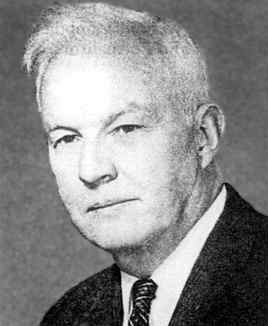
\includegraphics[width=0.6\textwidth]{Curry.jpeg}\\
    Haskell Curry {\scriptsize\emph (Image by University of St. Andrews)}\\[3mm]
  \end{marginfigure}
  \begin{marginfigure}
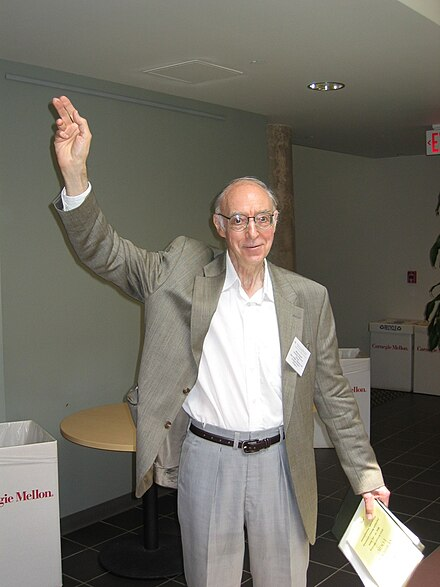
\includegraphics[width=0.6\textwidth]{William_Alvin_Howard_May_2004.jpg}\\
    William Alvin Howard {\scriptsize\emph (Image by Wikipedia)}\\[3mm]
  \end{marginfigure}

Hoewel sequenten-calculus en natuurlijke deductie uiteindelijk dezelfde logische stellingen kunnen bewijzen, en een bewijs met sequenten-calculus vaak eenvoudiger te vinden is door het methodisch toepassen van regels, is er een goede reden om natuurlijke deductie in te zetten: bewijzen met natuurlijke deductie tonen een \'e\'en-op\'e\'en overeenkomst (een \emph{isomorfisme} met computerprogramma's. Dat wil zeggen dat een bewijs direct vertaald kan worden naar een programma, dat daarmee door de computer geverifieerd kan worden, en dat we (in de juiste context) programma's niet hoeven te testen, maar de correctheid wiskundig kunnen bewijzen. Het isomorfisme toont zich daarnaast op een tweede niveau, in een directe overeenkomst tussen typen en logische formules. De overeenkomst is ontdekt door de Amerikaanse wiskundige en computer-wetenschapper Haskell Curry en de logicus William Alvin Howard, in eerste instantie in termen van Intuitionistische Logica (zie Sectie~\ref{sec:il}) en Curry's \emph{Lambda Calculus}\sidenote{De Lambda calculus vormt de basis voor het functionele programmeerparadigma, dat verschilt van imperatieve code zoals we die uit Python gewend zijn doordat alles als onveranderbaar wordt beschouwd. Dit geeft een meer wiskundige manier van programmeren, waar de focus ligt op het combineren van functies en recursie de plaats van loops inneemt. Dankzij het Curry-Howard isomorfisme is getypeerde functionele code vaak aanzienlijk minder gevoelig voor bugs.}, maar uit verder onderzoek is voor vrijwel iedere consistente logica een programmeer-tegenhanger bestond (en vice versa). In de tabel hieronder staat een selectie van termen die met behulp van het isomorfisme vertaald kunnen worden; dit biedt de mogelijkheid om kennis uit verschillende onderzoeksgebieden met elkaar te combineren.\\[5mm]

\begin{tabular}{l l}
  \bf Logica & \bf Programmeren \\
  Implicatie & Functietype \\
  Conjunctie & Producttypes (tuples) \\
  Disjunctie & Somtypes (disjunctive union) \\
  $\top$ & Unit-type \\
  $\bot$ & Leeg type \\
  Universele kwantor & $\Pi$-type \\
  Existenti\"ele kwantor & $\Sigma$-type \\
  Hypothesen & Vrije variabelen \\
  Implicatie-eliminatie & Functie-applicatie \\
  Implicatie-introductie & Abstractie \\
  Wet van Peirce (klassieke logica) & voortzettings-manipulatie \\
\end{tabular}\\[5mm]


\begin{aside}[Curry-Howard-Lambek en HoTT]
  \begin{marginfigure}
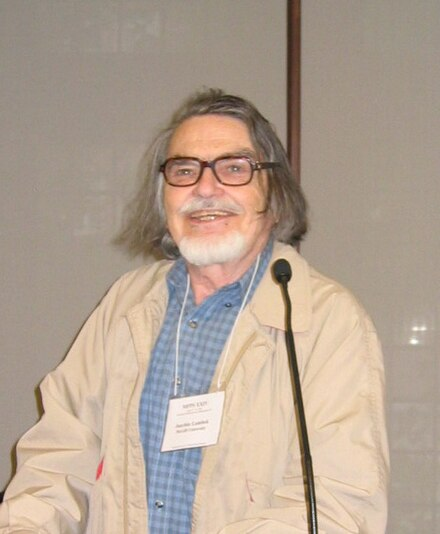
\includegraphics[width=0.6\textwidth]{Lambek_Joachim.jpg}\\
    Joachim Lambek {\scriptsize\emph (Image by Wikipedia)}\\[3mm]
  \end{marginfigure}

  In de jaren '70 koppelde Joachim Lambek het Curry-Howard isomorfisme via \emph{Cartesiaanse gesloten categorie\"en} aan de Categorie-theorie, een abstract maar erg krachtig wiskundige onderzoeksveld, waarbij gekeken wordt naar functies tussen objecten (zoals we dat ook met verzamelingen hebben gezien), maar dan zonder de interne elementen van een verzameling te beschouwen. Met wat slimme wiskundige trucs kunnen we toch heel veel over objecten zeggen zonder \enquote{erin} te mogen kijken, wat tot theori\"en leidt die heel breed toepasbaar zijn. Ze kunnen immers niet op inwendige details berusten, zolang ze hier niets van af weten. Inzichten die hiermee zijn opgedaan zijn van fundamenteel belang in experimentele programmeertalen. Met het werk van Lambek is het mogelijk alle begrippen uit logica en programmeer- en type-theorie in verband te brengen met nog breder wiskundig onderzoek.

  \begin{marginfigure}
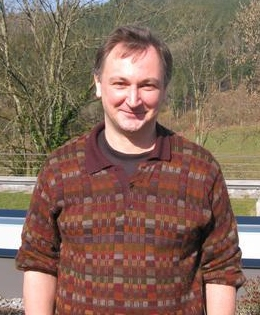
\includegraphics[width=0.6\textwidth]{VladimirVoevodsky.jpg}\\
    Vladimir Voevodsky {\scriptsize\emph (Image by Wikipedia)}\\[3mm]
  \end{marginfigure}

Inmiddels is door Vladimir Voevodsky op deze drie-eenheid doorgebouwd in de \emph{Homotopie Type-theorie}, waarmee hij een nieuw fundament onder de wiskunde probeerde te leggen op basis van computatie en formele software. Homotopie als wiskundig begrip gaat over een zekere zin van gelijkvormigheid van objecten, waarbij bepaalde transformaties zijn toegestaan; in dit geval zolang iets zonder knippen en plakken in elkaar te transformeren is --- denk aan een bal van klei, die je eenvoudig in een kubus kan vervormen. Wil je echter een donut maken, dan zul je een gat moeten cre\"eren en heb je de vorm fundamenteel veranderd. Deze vorm van gelijkheid vertaalt zich weer naar computerprogamma's: twee programma's met dezelfde code zijn zonder meer gelijk, maar wat als twee (qua code verschillende) programma's altijd dezelfde output en effecten hebben?
\end{aside}
